% Options for packages loaded elsewhere
\PassOptionsToPackage{unicode}{hyperref}
\PassOptionsToPackage{hyphens}{url}
%
\documentclass[
]{book}
\usepackage{lmodern}
\usepackage{amssymb,amsmath}
\usepackage{ifxetex,ifluatex}
\ifnum 0\ifxetex 1\fi\ifluatex 1\fi=0 % if pdftex
  \usepackage[T1]{fontenc}
  \usepackage[utf8]{inputenc}
  \usepackage{textcomp} % provide euro and other symbols
\else % if luatex or xetex
  \usepackage{unicode-math}
  \defaultfontfeatures{Scale=MatchLowercase}
  \defaultfontfeatures[\rmfamily]{Ligatures=TeX,Scale=1}
\fi
% Use upquote if available, for straight quotes in verbatim environments
\IfFileExists{upquote.sty}{\usepackage{upquote}}{}
\IfFileExists{microtype.sty}{% use microtype if available
  \usepackage[]{microtype}
  \UseMicrotypeSet[protrusion]{basicmath} % disable protrusion for tt fonts
}{}
\makeatletter
\@ifundefined{KOMAClassName}{% if non-KOMA class
  \IfFileExists{parskip.sty}{%
    \usepackage{parskip}
  }{% else
    \setlength{\parindent}{0pt}
    \setlength{\parskip}{6pt plus 2pt minus 1pt}}
}{% if KOMA class
  \KOMAoptions{parskip=half}}
\makeatother
\usepackage{xcolor}
\IfFileExists{xurl.sty}{\usepackage{xurl}}{} % add URL line breaks if available
\IfFileExists{bookmark.sty}{\usepackage{bookmark}}{\usepackage{hyperref}}
\hypersetup{
  pdftitle={Computing},
  pdfauthor={Bill Last Updated:},
  hidelinks,
  pdfcreator={LaTeX via pandoc}}
\urlstyle{same} % disable monospaced font for URLs
\usepackage{color}
\usepackage{fancyvrb}
\newcommand{\VerbBar}{|}
\newcommand{\VERB}{\Verb[commandchars=\\\{\}]}
\DefineVerbatimEnvironment{Highlighting}{Verbatim}{commandchars=\\\{\}}
% Add ',fontsize=\small' for more characters per line
\usepackage{framed}
\definecolor{shadecolor}{RGB}{248,248,248}
\newenvironment{Shaded}{\begin{snugshade}}{\end{snugshade}}
\newcommand{\AlertTok}[1]{\textcolor[rgb]{0.94,0.16,0.16}{#1}}
\newcommand{\AnnotationTok}[1]{\textcolor[rgb]{0.56,0.35,0.01}{\textbf{\textit{#1}}}}
\newcommand{\AttributeTok}[1]{\textcolor[rgb]{0.77,0.63,0.00}{#1}}
\newcommand{\BaseNTok}[1]{\textcolor[rgb]{0.00,0.00,0.81}{#1}}
\newcommand{\BuiltInTok}[1]{#1}
\newcommand{\CharTok}[1]{\textcolor[rgb]{0.31,0.60,0.02}{#1}}
\newcommand{\CommentTok}[1]{\textcolor[rgb]{0.56,0.35,0.01}{\textit{#1}}}
\newcommand{\CommentVarTok}[1]{\textcolor[rgb]{0.56,0.35,0.01}{\textbf{\textit{#1}}}}
\newcommand{\ConstantTok}[1]{\textcolor[rgb]{0.00,0.00,0.00}{#1}}
\newcommand{\ControlFlowTok}[1]{\textcolor[rgb]{0.13,0.29,0.53}{\textbf{#1}}}
\newcommand{\DataTypeTok}[1]{\textcolor[rgb]{0.13,0.29,0.53}{#1}}
\newcommand{\DecValTok}[1]{\textcolor[rgb]{0.00,0.00,0.81}{#1}}
\newcommand{\DocumentationTok}[1]{\textcolor[rgb]{0.56,0.35,0.01}{\textbf{\textit{#1}}}}
\newcommand{\ErrorTok}[1]{\textcolor[rgb]{0.64,0.00,0.00}{\textbf{#1}}}
\newcommand{\ExtensionTok}[1]{#1}
\newcommand{\FloatTok}[1]{\textcolor[rgb]{0.00,0.00,0.81}{#1}}
\newcommand{\FunctionTok}[1]{\textcolor[rgb]{0.00,0.00,0.00}{#1}}
\newcommand{\ImportTok}[1]{#1}
\newcommand{\InformationTok}[1]{\textcolor[rgb]{0.56,0.35,0.01}{\textbf{\textit{#1}}}}
\newcommand{\KeywordTok}[1]{\textcolor[rgb]{0.13,0.29,0.53}{\textbf{#1}}}
\newcommand{\NormalTok}[1]{#1}
\newcommand{\OperatorTok}[1]{\textcolor[rgb]{0.81,0.36,0.00}{\textbf{#1}}}
\newcommand{\OtherTok}[1]{\textcolor[rgb]{0.56,0.35,0.01}{#1}}
\newcommand{\PreprocessorTok}[1]{\textcolor[rgb]{0.56,0.35,0.01}{\textit{#1}}}
\newcommand{\RegionMarkerTok}[1]{#1}
\newcommand{\SpecialCharTok}[1]{\textcolor[rgb]{0.00,0.00,0.00}{#1}}
\newcommand{\SpecialStringTok}[1]{\textcolor[rgb]{0.31,0.60,0.02}{#1}}
\newcommand{\StringTok}[1]{\textcolor[rgb]{0.31,0.60,0.02}{#1}}
\newcommand{\VariableTok}[1]{\textcolor[rgb]{0.00,0.00,0.00}{#1}}
\newcommand{\VerbatimStringTok}[1]{\textcolor[rgb]{0.31,0.60,0.02}{#1}}
\newcommand{\WarningTok}[1]{\textcolor[rgb]{0.56,0.35,0.01}{\textbf{\textit{#1}}}}
\usepackage{longtable,booktabs}
% Correct order of tables after \paragraph or \subparagraph
\usepackage{etoolbox}
\makeatletter
\patchcmd\longtable{\par}{\if@noskipsec\mbox{}\fi\par}{}{}
\makeatother
% Allow footnotes in longtable head/foot
\IfFileExists{footnotehyper.sty}{\usepackage{footnotehyper}}{\usepackage{footnote}}
\makesavenoteenv{longtable}
\usepackage{graphicx,grffile}
\makeatletter
\def\maxwidth{\ifdim\Gin@nat@width>\linewidth\linewidth\else\Gin@nat@width\fi}
\def\maxheight{\ifdim\Gin@nat@height>\textheight\textheight\else\Gin@nat@height\fi}
\makeatother
% Scale images if necessary, so that they will not overflow the page
% margins by default, and it is still possible to overwrite the defaults
% using explicit options in \includegraphics[width, height, ...]{}
\setkeys{Gin}{width=\maxwidth,height=\maxheight,keepaspectratio}
% Set default figure placement to htbp
\makeatletter
\def\fps@figure{htbp}
\makeatother
\setlength{\emergencystretch}{3em} % prevent overfull lines
\providecommand{\tightlist}{%
  \setlength{\itemsep}{0pt}\setlength{\parskip}{0pt}}
\setcounter{secnumdepth}{5}
\usepackage{booktabs}
\usepackage{amsthm}
\makeatletter
\def\thm@space@setup{%
  \thm@preskip=8pt plus 2pt minus 4pt
  \thm@postskip=\thm@preskip
}
\makeatother
\usepackage[]{natbib}
\bibliographystyle{apalike}

\title{Computing}
\author{Bill Last Updated:}
\date{15 February, 2020}

\begin{document}
\frontmatter
\maketitle

{
\setcounter{tocdepth}{1}
\tableofcontents
}
\mainmatter
\hypertarget{my-section}{%
\chapter*{Preface: Motivation}\label{my-section}}
\addcontentsline{toc}{chapter}{Preface: Motivation}

All the notes I have done here are about computing. While I have tried my best, probably there are still some typos and errors. Please feel free to let me know in case you find one. Thank you!

\hypertarget{monte-carlo-approximation}{%
\chapter{Monte carlo approximation}\label{monte-carlo-approximation}}

Since GLMM can use EM algorithm in its maximum likelihood calculation (see McCulloch, 1994), it is practically useful to rehearse EM and other computing techniques.

Example: calculate the integral of \(p(z>2)\) when \(z \sim N(0,1)\). To use Monte Carlo approximation, we can have an indicator function, which will determine whether the sample from \(N(0,1)\) will be included into the calculation of the integral.

\begin{Shaded}
\begin{Highlighting}[]
\NormalTok{Nsim=}\DecValTok{10}\OperatorTok{^}\DecValTok{4}

\NormalTok{indicator=}\ControlFlowTok{function}\NormalTok{(x)\{}
\NormalTok{y=}\KeywordTok{ifelse}\NormalTok{((x}\OperatorTok{>}\DecValTok{2}\NormalTok{),}\DecValTok{1}\NormalTok{,}\DecValTok{0}\NormalTok{)}
\KeywordTok{return}\NormalTok{(y)\}}

\NormalTok{newdata<-}\KeywordTok{rnorm}\NormalTok{(Nsim, }\DecValTok{0}\NormalTok{,}\DecValTok{1}\NormalTok{ )}

\NormalTok{mc=}\KeywordTok{c}\NormalTok{(); v=}\KeywordTok{c}\NormalTok{(); upper=}\KeywordTok{c}\NormalTok{(); lower=}\KeywordTok{c}\NormalTok{()}

\ControlFlowTok{for}\NormalTok{ (j }\ControlFlowTok{in} \DecValTok{1}\OperatorTok{:}\NormalTok{Nsim)}
\NormalTok{\{}
\NormalTok{mc[j]=}\KeywordTok{mean}\NormalTok{(}\KeywordTok{indicator}\NormalTok{(newdata[}\DecValTok{1}\OperatorTok{:}\NormalTok{j]))}
\NormalTok{v[j]=(j}\OperatorTok{^}\NormalTok{\{}\OperatorTok{-}\DecValTok{1}\NormalTok{\})}\OperatorTok{*}\KeywordTok{var}\NormalTok{(}\KeywordTok{indicator}\NormalTok{(newdata[}\DecValTok{1}\OperatorTok{:}\NormalTok{j]))}
\NormalTok{upper[j]=mc[j]}\OperatorTok{+}\FloatTok{1.96}\OperatorTok{*}\KeywordTok{sqrt}\NormalTok{(v[j])}
\NormalTok{lower[j]=mc[j]}\OperatorTok{-}\FloatTok{1.96}\OperatorTok{*}\KeywordTok{sqrt}\NormalTok{(v[j])}
\NormalTok{\}}

\KeywordTok{library}\NormalTok{(ggplot2)}
\NormalTok{values=}\KeywordTok{c}\NormalTok{(mc,upper,lower)}
\NormalTok{type=}\KeywordTok{c}\NormalTok{(}\KeywordTok{rep}\NormalTok{(}\StringTok{"mc"}\NormalTok{,Nsim),}\KeywordTok{rep}\NormalTok{(}\StringTok{"upper"}\NormalTok{,Nsim),}\KeywordTok{rep}\NormalTok{(}\StringTok{"lower"}\NormalTok{,Nsim))}
\NormalTok{iter=}\KeywordTok{rep}\NormalTok{(}\KeywordTok{seq}\NormalTok{(}\DecValTok{1}\OperatorTok{:}\NormalTok{Nsim),}\DecValTok{3}\NormalTok{)}
\NormalTok{data=}\KeywordTok{data.frame}\NormalTok{(}\DataTypeTok{val=}\NormalTok{values, }\DataTypeTok{tp=}\NormalTok{type, }\DataTypeTok{itr=}\NormalTok{iter)}
\NormalTok{Rcode<-}\KeywordTok{ggplot}\NormalTok{(data,}\KeywordTok{aes}\NormalTok{(itr,val,}\DataTypeTok{col=}\NormalTok{tp))}\OperatorTok{+}\KeywordTok{geom_line}\NormalTok{(}\DataTypeTok{size=}\FloatTok{0.5}\NormalTok{)}
\NormalTok{Rcode}\OperatorTok{+}\KeywordTok{geom_hline}\NormalTok{(}\DataTypeTok{yintercept=}\DecValTok{1}\OperatorTok{-}\KeywordTok{pnorm}\NormalTok{(}\DecValTok{2}\NormalTok{),}\DataTypeTok{color=}\StringTok{"green"}\NormalTok{,}\DataTypeTok{size=}\FloatTok{0.5}\NormalTok{)}
\end{Highlighting}
\end{Shaded}

\begin{verbatim}
## Warning: Removed 2 rows containing missing values (geom_path).
\end{verbatim}

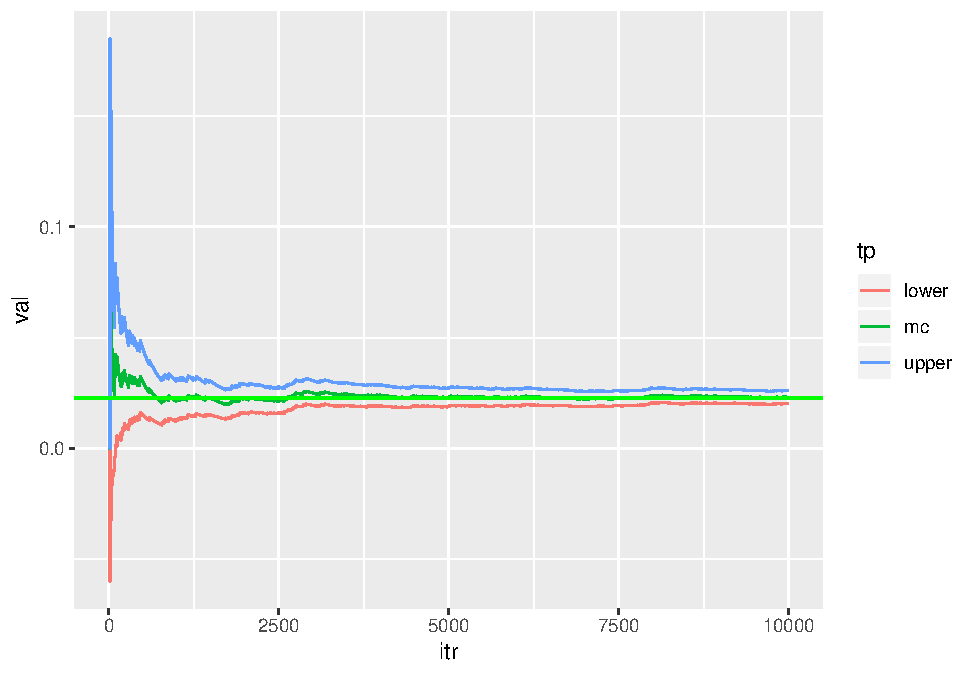
\includegraphics{bookdown-demo_files/figure-latex/unnamed-chunk-1-1.pdf}

\hypertarget{importance-sampling}{%
\chapter{Importance sampling}\label{importance-sampling}}

Importance sampling has samples generated from a different distribution than the distribution of interest. Specifically, assume that we want to calculate the expected value of \(h(x)\), and \(x \sim f(x)\).

\[E(h(x))=\int h(x) f(x) dx = \int h(x) \frac{f(x)}{g(x)} g(x) dx \]
We can sample \(x_i\) from \(g(x)\) and then calculate the mean of \(h(x_i) \frac{f(x_i)}{g(x_i)}\).

Using the same explane above, we can use a shifted exponential distribution to help calculate the intergral for normal distribution. Specifically,

\[\int_2^{\infty} \frac{1}{2 \pi} e^{-\frac{1}{2}x^2}dx = \int_2^{\infty} \frac{\frac{1}{2 \pi} e^{-\frac{1}{2}x^2}}{e^{-(x-2)}} e^{-(x-2)}dx \]
The idea is that, we can generate \(x_i\) from exponential distribution of \(e^{-(x-2)}\), and then insert them into the targeted ``expected (value) function'' of \(\frac{\frac{1}{2 \pi} e^{-\frac{1}{2}x^2}}{e^{-(x-2)}}\). Thus, as you can see, importance sampling is based on the law of large numbers (i.e., If the same experiment or study is repeated independently a large number of times, the average of the results of the trials must be close to the expected value). We can use it to calculate integral based on link of the definition of expected value.

\begin{Shaded}
\begin{Highlighting}[]
\NormalTok{Nsim=}\DecValTok{10}\OperatorTok{^}\DecValTok{4}
\NormalTok{normal_density=}\ControlFlowTok{function}\NormalTok{(x)}
\NormalTok{\{y=(}\DecValTok{1}\OperatorTok{/}\KeywordTok{sqrt}\NormalTok{(}\DecValTok{2}\OperatorTok{*}\NormalTok{pi))}\OperatorTok{*}\KeywordTok{exp}\NormalTok{(}\OperatorTok{-}\FloatTok{0.5}\OperatorTok{*}\NormalTok{(x}\OperatorTok{^}\DecValTok{2}\NormalTok{))}
\KeywordTok{return}\NormalTok{(y)\}}
\NormalTok{x=}\DecValTok{2}\OperatorTok{-}\KeywordTok{log}\NormalTok{(}\KeywordTok{runif}\NormalTok{(Nsim))}
\NormalTok{ImpS=}\KeywordTok{c}\NormalTok{(); v=}\KeywordTok{c}\NormalTok{(); upper=}\KeywordTok{c}\NormalTok{(); lower=}\KeywordTok{c}\NormalTok{()}
\ControlFlowTok{for}\NormalTok{ (j }\ControlFlowTok{in} \DecValTok{1}\OperatorTok{:}\NormalTok{Nsim)}
\NormalTok{\{}
\NormalTok{ImpS[j]=}\KeywordTok{mean}\NormalTok{(}\KeywordTok{normal_density}\NormalTok{(x[}\DecValTok{1}\OperatorTok{:}\NormalTok{j])}\OperatorTok{/}\KeywordTok{exp}\NormalTok{(}\OperatorTok{-}\NormalTok{(x[}\DecValTok{1}\OperatorTok{:}\NormalTok{j]}\OperatorTok{-}\DecValTok{2}\NormalTok{)))}
\NormalTok{v[j]=(j}\OperatorTok{^}\NormalTok{\{}\OperatorTok{-}\DecValTok{1}\NormalTok{\})}\OperatorTok{*}\KeywordTok{var}\NormalTok{(}\KeywordTok{normal_density}\NormalTok{(x[}\DecValTok{1}\OperatorTok{:}\NormalTok{j])}\OperatorTok{/}\KeywordTok{exp}\NormalTok{(}\OperatorTok{-}\NormalTok{(x[}\DecValTok{1}\OperatorTok{:}\NormalTok{j]}\OperatorTok{-}\DecValTok{2}\NormalTok{)))}
\NormalTok{upper[j]=ImpS[j]}\OperatorTok{+}\FloatTok{1.96}\OperatorTok{*}\KeywordTok{sqrt}\NormalTok{(v[j])}
\NormalTok{lower[j]=ImpS[j]}\OperatorTok{-}\FloatTok{1.96}\OperatorTok{*}\KeywordTok{sqrt}\NormalTok{(v[j])}
\NormalTok{\}}

\KeywordTok{library}\NormalTok{(ggplot2)}
\NormalTok{values=}\KeywordTok{c}\NormalTok{(ImpS,upper,lower)}
\NormalTok{type=}\KeywordTok{c}\NormalTok{(}\KeywordTok{rep}\NormalTok{(}\StringTok{"mc"}\NormalTok{,Nsim),}\KeywordTok{rep}\NormalTok{(}\StringTok{"upper"}\NormalTok{,Nsim),}\KeywordTok{rep}\NormalTok{(}\StringTok{"lower"}\NormalTok{,Nsim))}
\NormalTok{iter=}\KeywordTok{rep}\NormalTok{(}\KeywordTok{seq}\NormalTok{(}\DecValTok{1}\OperatorTok{:}\NormalTok{Nsim),}\DecValTok{3}\NormalTok{)}
\NormalTok{data=}\KeywordTok{data.frame}\NormalTok{(}\DataTypeTok{val=}\NormalTok{values, }\DataTypeTok{tp=}\NormalTok{type, }\DataTypeTok{itr=}\NormalTok{iter)}
\KeywordTok{ggplot}\NormalTok{(data,}\KeywordTok{aes}\NormalTok{(itr,val,}\DataTypeTok{col=}\NormalTok{tp))}\OperatorTok{+}\KeywordTok{geom_line}\NormalTok{(}\DataTypeTok{size=}\FloatTok{0.5}\NormalTok{)}\OperatorTok{+}
\KeywordTok{geom_hline}\NormalTok{(}\DataTypeTok{yintercept=}\DecValTok{1}\OperatorTok{-}\KeywordTok{pnorm}\NormalTok{(}\DecValTok{2}\NormalTok{),}\DataTypeTok{color=}\StringTok{"green"}\NormalTok{,}\DataTypeTok{size=}\FloatTok{0.5}\NormalTok{)}
\end{Highlighting}
\end{Shaded}

\begin{verbatim}
## Warning: Removed 2 rows containing missing values (geom_path).
\end{verbatim}

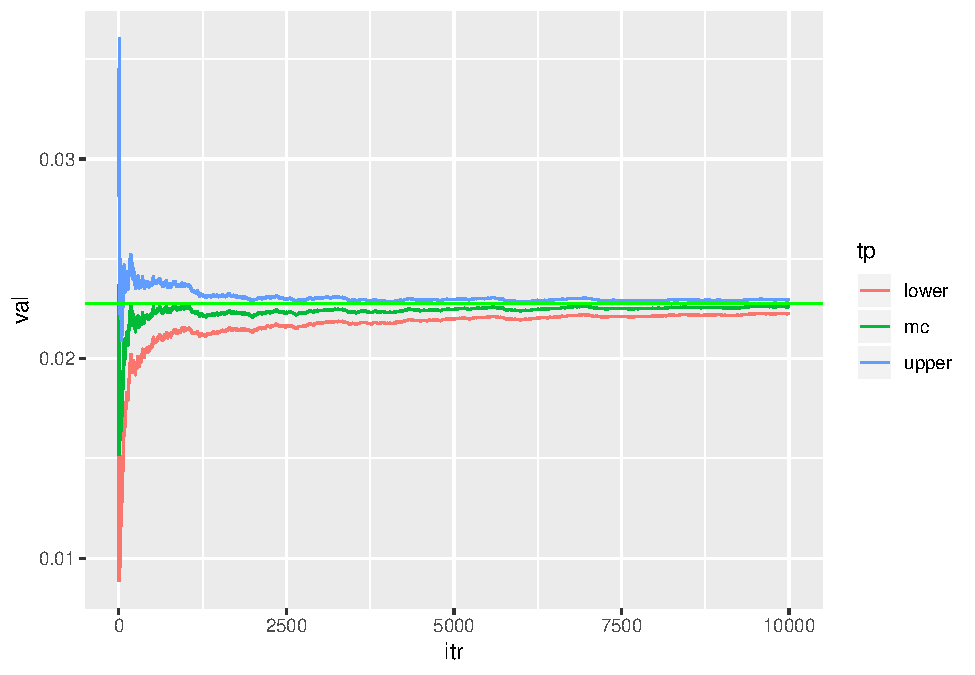
\includegraphics{bookdown-demo_files/figure-latex/unnamed-chunk-2-1.pdf}

\hypertarget{newton-raphson-algorithm}{%
\chapter{Newton Raphson algorithm}\label{newton-raphson-algorithm}}

The main purpose of Newton Raphson algorithm is to calculate the root of a function (e.g., \(x^2-3=0\)). We know that in order to maximize the MLE, we need to calculate the first derivatice of the function and then set it to zero \(\ell^{'}(x)=0\). Thus, we can use the same Newton Raphson method to help calculate the MLE maximization as well.

There are different ways to understand Newton Raphson method, but I found the method fo geometric the most easy way to explain.

\begin{figure}
\centering
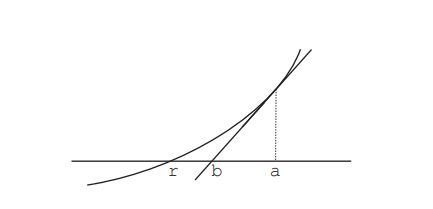
\includegraphics{Newton.jpg}
\caption{Credit of this figure: \url{https://www.math.ubc.ca/~anstee/math104/newtonmethod.pdf}}
\end{figure}

Specifically, suppose that you want to calculate the root of a function \(f(x)=0\). We assume the root is \(r\). However, we do not know that, and we randomly guess a point of \(a\). Thus, we can get a tangent line with slope of \(f^{'}(a)\) and a point of \((a,f(a))\). Since we know the slope and one of its points, we can write the function for this tangent line.

\[y-f(a)=f^{'}(a)(x-a)\]
To calculate the \(x-intercept\), namely \(b\) in the figure, we can set \(y=0\), and get the following:

\[-f(a)=f^{'}(a)(x-a) \Rightarrow x (or, b)= a-\frac{f(a)}{f^{'}(a)}\]
If there is significant difference of \(|a-b|\), we know that our orginal guess of \(a\) is not good. We better use \(b\) as the next guess, and calculate its tangent line again. To generalize, we can write it as follows.
\[x_{t+1}=x_{t}-\frac{f(x_t)}{f^{'}(x_t)}\]

Okay, this method above is to calculate the root. For MLE, we can also use this method to calculate the root for the \(\ell ^{'}=0\). We can write it as follows.

\[x_{t+1}=x_{t}-\frac{\ell^{'}(x_t)}{\ell^{''}(x_t)}\]
Often, \(x\) is not just a single unknow parameter, but a vector. For this case, we can write it as follows.

\[\beta_{t+1}=\beta_{t}-\frac{\ell^{'}(\beta_t)}{\ell^{''}(\beta_t)}\]

\hypertarget{calculate-the-root}{%
\subsection{Calculate the root}\label{calculate-the-root}}

\(x^3-5=0\)

Note that, this is obviously not a maximization problem. In contrast, it involves a function with zero. As we can see, we can think it as the first order of Taylor approximation. That is, \(f^{'}(x)=x^3-5=0\). As we can see the following plot, it converts very quickly.

\begin{Shaded}
\begin{Highlighting}[]
\NormalTok{f_firstorder=}\ControlFlowTok{function}\NormalTok{(x)\{x}\OperatorTok{^}\DecValTok{3-5}\NormalTok{\}}
\NormalTok{f_secondorder=}\ControlFlowTok{function}\NormalTok{(x)\{}\DecValTok{3}\OperatorTok{*}\NormalTok{x\}}
\NormalTok{x_old=}\DecValTok{1}\NormalTok{;tolerance=}\FloatTok{1e-3}
\NormalTok{max_its=}\DecValTok{2000}\NormalTok{;iteration=}\DecValTok{1}\NormalTok{;difference=}\DecValTok{2}
\NormalTok{c_iteration<-}\KeywordTok{c}\NormalTok{() }\CommentTok{## to collect numbers generated in the iteration process }
\ControlFlowTok{while}\NormalTok{(difference}\OperatorTok{>}\NormalTok{tolerance }\OperatorTok{&}\StringTok{ }\NormalTok{iteration}\OperatorTok{<}\NormalTok{max_its)\{}
\NormalTok{  x_updated=x_old}\OperatorTok{-}\NormalTok{(}\KeywordTok{f_firstorder}\NormalTok{(x_old)}\OperatorTok{/}\KeywordTok{f_secondorder}\NormalTok{(x_old))}
\NormalTok{  difference=}\KeywordTok{abs}\NormalTok{(x_updated}\OperatorTok{-}\NormalTok{x_old);}
\NormalTok{  iteration=iteration}\OperatorTok{+}\DecValTok{1}\NormalTok{;}
\NormalTok{  x_old=x_updated}
\NormalTok{  c_iteration<-}\KeywordTok{c}\NormalTok{(c_iteration,x_updated)\}}

\KeywordTok{plot}\NormalTok{(c_iteration,}\DataTypeTok{type=}\StringTok{"b"}\NormalTok{)}
\end{Highlighting}
\end{Shaded}

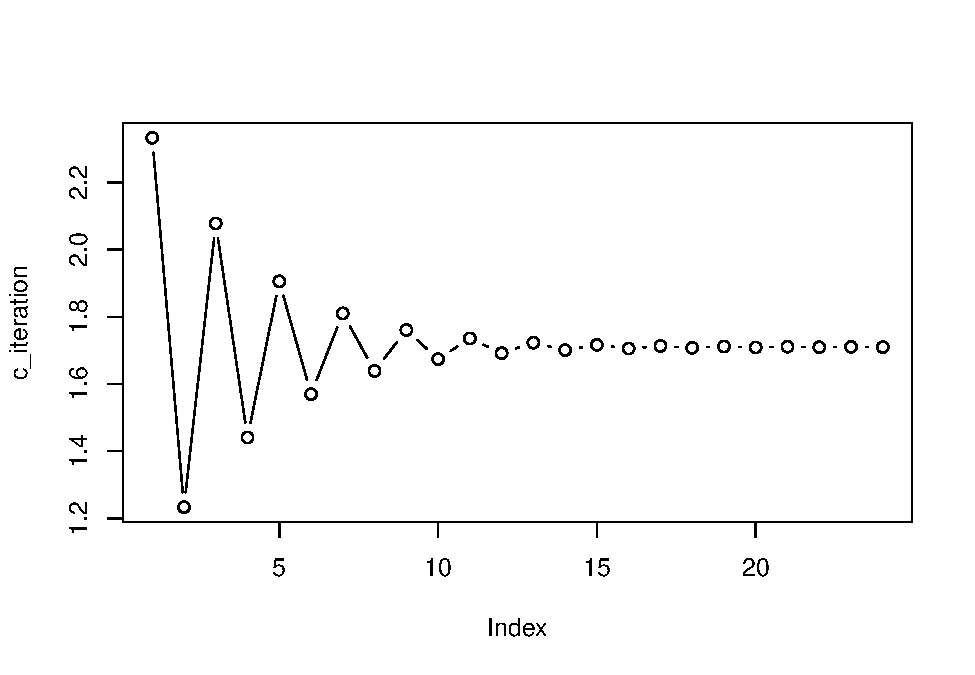
\includegraphics{bookdown-demo_files/figure-latex/unnamed-chunk-3-1.pdf}

\hypertarget{logistic-regression}{%
\subsection{Logistic regression}\label{logistic-regression}}

Suppose we have \(n\) observation, and \(m\) variables.

\[\begin{bmatrix}
x_{11} & x_{12} & x_{13} & ... & x_{1m}\\
x_{21} & x_{22} & x_{23} & ... & x_{2m} \\
...\\
x_{n1} & x_{n2} & x_{n3} & ... & x_{nm}
\end{bmatrix}\]

Typically, we add a vector of \(1\) being used to estimate the constant.

\[\begin{bmatrix}
1 & x_{11} & x_{12} & x_{13} & ... & x_{1m}\\
1 & x_{21} & x_{22} & x_{23} & ... & x_{2m} \\
...\\
1 & x_{n1} & x_{n2} & x_{n3} & ... & x_{nm}
\end{bmatrix}\]

And, we have observe a vector of \(n\) \(y_i\) as well, which is a binary variable:

\[Y = \begin{bmatrix}1 \\
0 \\
1 \\
0 \\
0 \\
0 \\
...\\
1 \\
\end{bmatrix}\]

Using the content from the MLE chapter, we can get:

\[\mathbf{L}=\prod_{i=1}^{n} p_i^{ y_i}(1-p_i)^{(1-y_i)}\]

Further, we can get a log-transformed format.

\[log (\mathbf{L})=\sum_{i=1}^{n}[y_i log (p_i) + (1-y_i) log(1-p_i)]\]
Given that \(p_i=\frac{e^{\beta_0+\beta_1x_1+...+\beta_nx_n}}{1+e^{\beta_0+\beta_1x_1+...+\beta_nx_n}}=\frac{e^{\beta^Tx}}{1+e^{\beta^Tx}}\), we can rewrite it as follows:

\[log (\mathbf{L})=\ell=\sum_{i=1}^{n}[y_i log (\frac{e^{\beta^Tx_i}}{1+e^{\beta^Tx_i}}) + (1-y_i) log(1-\frac{e^{\beta^Tx_i}}{1+e^{\beta^Tx_i}})]\]
Before doing the derivative, we set.
\[\frac{e^{\beta^Tx_i}}{1+e^{\beta^Tx_i}} = p(\beta ^T x_i)\]

\[log (\mathbf{L})=\ell=\sum_{i=1}^{n}[y_i log (p(\beta ^T x_i)) + (1-y_i) log(1-p(\beta ^T x_i))]\]

Note that, \(\frac{\partial p(\beta ^T x_i)}{\partial (\beta ^T x_i)} = p(\beta ^T x_i)(1-p(\beta ^T x_i))\). We will use it later.

\[\begin{aligned}
\nabla \ell &= \sum_{i=1}^{n} [y_i \frac{1}{p(\beta ^T x_i)} \frac{\partial p(\beta ^T x_i)}{\partial (\beta ^T x_i)}\frac{\partial (\beta ^T x_i)}{\partial \beta}+(1-y_i) \frac{1}{1-p(\beta ^T x_i)}(-1)\frac{\partial p(\beta ^T x_i)}{\partial (\beta ^T x_i)}\frac{\partial (\beta ^T x_i)}{\partial \beta}] \\
&= \sum_{i=1}^{n} x_i^T[y_i \frac{1}{p(\beta ^T x_i)} p(\beta ^T x_i)(1-p(\beta ^T x_i))+(1-y_i) \frac{1}{1-p(\beta ^T x_i)}(-1)p(\beta ^T x_i)(1-p(\beta ^T x_i))] \\
&= \sum_{i=1}^{n} x_i^T[y_i \frac{1}{p(\beta ^T x_i)} p(\beta ^T x_i)(1-p(\beta ^T x_i))-(1-y_i) \frac{1}{1-p(\beta ^T x_i)}p(\beta ^T x_i)(1-p(\beta ^T x_i))] \\
&= \sum_{i=1}^{n} x_i^T[y_i (1-p(\beta ^T x_i))-(1-y_i) p(\beta ^T x_i)] \\
&=\sum_{i=1}^{n} x_i^T[y_i-y_ip(\beta ^T x_i)-p(\beta ^T x_i)+y_i p(\beta ^T x_i)] \\
&=\sum_{i=1}^{n} x_i^T[y_i-p(\beta ^T x_i)] \\
&= \sum_{i=1}^{n} x_i^T[y_i-\frac{e^{\beta^Tx_i}}{1+e^{\beta^Tx_i}}]
\end{aligned}\]

As noted, the Newton Raphson algorithm needs the second order.

\[\begin{aligned}
\nabla^2 \ell &=\frac{\partial \sum_{i=1}^{n} x_i^T[y_i-p(\beta ^T x_i)]}{\partial \beta} \\
&=-\sum_{i=1}^{n} x_i^T\frac{\partial p(\beta ^T x_i) }{\partial \beta}\\
&=-\sum_{i=1}^{n} x_i^T\frac{\partial p(\beta ^T x_i) }{\partial (\beta^Tx_i)} \frac{\partial (\beta^Tx_i)}{\partial \beta}\\
&=-\sum_{i=1}^{n} x_i^T p(\beta ^T x_i)(1-p(\beta ^T x_i))x_i
\end{aligned}\]

The following are the data simulation (3 IVs and 1 DV) and Newton Raphson analysis.

\begin{Shaded}
\begin{Highlighting}[]
\CommentTok{# Data generation}
\KeywordTok{set.seed}\NormalTok{(}\DecValTok{123}\NormalTok{)}
\NormalTok{n=}\DecValTok{500}
\NormalTok{x1_norm<-}\KeywordTok{rnorm}\NormalTok{(n)}
\NormalTok{x2_norm<-}\KeywordTok{rnorm}\NormalTok{(n,}\DecValTok{3}\NormalTok{,}\DecValTok{4}\NormalTok{)}
\NormalTok{x3_norm<-}\KeywordTok{rnorm}\NormalTok{(n,}\DecValTok{4}\NormalTok{,}\DecValTok{6}\NormalTok{)}
\NormalTok{x_combined<-}\KeywordTok{cbind}\NormalTok{(}\DecValTok{1}\NormalTok{,x1_norm,x2_norm,x3_norm) }\CommentTok{# dimension: n*4}
\NormalTok{coefficients_new<-}\KeywordTok{c}\NormalTok{(}\DecValTok{1}\NormalTok{,}\DecValTok{2}\NormalTok{,}\DecValTok{3}\NormalTok{,}\DecValTok{4}\NormalTok{)  }\CommentTok{#true regression coefficient}
\NormalTok{inv_logit<-}\ControlFlowTok{function}\NormalTok{(x,b)\{}\KeywordTok{exp}\NormalTok{(x}\OperatorTok\NormalTok{b)}\OperatorTok{/}\NormalTok{(}\DecValTok{1}\OperatorTok{+}\KeywordTok{exp}\NormalTok{(x}\OperatorTok\NormalTok{b))\}}
\NormalTok{prob_generated<-}\KeywordTok{inv_logit}\NormalTok{(x_combined,coefficients_new)}
\NormalTok{y<-}\KeywordTok{c}\NormalTok{()}
\ControlFlowTok{for}\NormalTok{ (i }\ControlFlowTok{in} \DecValTok{1}\OperatorTok{:}\NormalTok{n) \{y[i]<-}\KeywordTok{rbinom}\NormalTok{(}\DecValTok{1}\NormalTok{,}\DecValTok{1}\NormalTok{,prob_generated[i])\}}

\CommentTok{# Newton Raphson}

\CommentTok{#We need to set random starting values.}
\NormalTok{beta_old<-}\KeywordTok{c}\NormalTok{(}\DecValTok{1}\NormalTok{,}\DecValTok{1}\NormalTok{,}\DecValTok{1}\NormalTok{,}\DecValTok{1}\NormalTok{)}
\NormalTok{tolerance=}\FloatTok{1e-3}
\NormalTok{max_its=}\DecValTok{2000}\NormalTok{;iteration=}\DecValTok{1}\NormalTok{;difference=}\DecValTok{2}
\NormalTok{W<-}\KeywordTok{matrix}\NormalTok{(}\DecValTok{0}\NormalTok{,n,n)}

\ControlFlowTok{while}\NormalTok{(difference}\OperatorTok{>}\NormalTok{tolerance }\OperatorTok{&}\StringTok{ }\NormalTok{iteration}\OperatorTok{<}\NormalTok{max_its)}
\NormalTok{  \{}
  \CommentTok{# The first order}
\NormalTok{  f_firstorder<-}\KeywordTok{t}\NormalTok{(x_combined)}\OperatorTok\NormalTok{(y}\OperatorTok{-}\KeywordTok{inv_logit}\NormalTok{(x_combined,beta_old))}
  \CommentTok{# The second order}
  \KeywordTok{diag}\NormalTok{(W) =}\StringTok{ }\KeywordTok{inv_logit}\NormalTok{(x_combined,beta_old)}\OperatorTok{*}\NormalTok{(}\DecValTok{1}\OperatorTok{-}\KeywordTok{inv_logit}\NormalTok{(x_combined,beta_old))}
\NormalTok{  f_secondorder<-}\OperatorTok{-}\KeywordTok{t}\NormalTok{(x_combined)}\OperatorTok\NormalTok{W}\OperatorTok\NormalTok{x_combined}
  \CommentTok{# Calculate the beta_updated}
\NormalTok{  beta_updated=beta_old}\OperatorTok{-}\NormalTok{(}\KeywordTok{solve}\NormalTok{(f_secondorder)}\OperatorTok\NormalTok{f_firstorder)}
\NormalTok{  difference=}\KeywordTok{max}\NormalTok{(}\KeywordTok{abs}\NormalTok{(beta_updated}\OperatorTok{-}\NormalTok{beta_old));}
\NormalTok{  iteration=iteration}\OperatorTok{+}\DecValTok{1}\NormalTok{;}
\NormalTok{  beta_old=beta_updated\}}

\NormalTok{beta_old}
\end{Highlighting}
\end{Shaded}

\begin{verbatim}
##              [,1]
##         0.9590207
## x1_norm 1.7974165
## x2_norm 3.0072303
## x3_norm 3.9578107
\end{verbatim}

\hypertarget{metropolis-hastings}{%
\chapter{Metropolis Hastings}\label{metropolis-hastings}}

Metropolis--Hastings is a MCMC method for obtaining a sequence of random samples from a probability distribution from which direct sampling is difficult. By using the samples, we can plot the distribution (through histgram), or we can calculate the integral (e.g., you need to calculate the expected value).

(Side note: does this remind you the importance sampling? Very similiar!)

Basic logic (my own summary):

\begin{enumerate}
\def\labelenumi{(\arabic{enumi})}
\item
  Set up a random starting value of \(x_0\).
\item
  Sample a \(y_0\) from the instrumental function of \(q(x)\).
\item
  Calculate the following:
\end{enumerate}

\(p =\frac{f(y_0)}{f(x_0)}\frac{q(x_0)}{q(y_0)}\)

\begin{enumerate}
\def\labelenumi{(\arabic{enumi})}
\setcounter{enumi}{3}
\item
  \(\rho=min(p, 1)\)
\item
  \(x_{1}=\begin{cases} y_0 & p \\ x_0 & 1-p \end{cases}\)
\item
  Repeat \(n\) times (\(n\) is set subjectively.)
\end{enumerate}

Use normal pdf to sample gamma distribution

\begin{Shaded}
\begin{Highlighting}[]
\NormalTok{alpha=}\FloatTok{2.7}\NormalTok{; beta=}\FloatTok{6.3} \CommentTok{# I randomly chose alpha and beta values for the target gamma function}

\NormalTok{Nsim=}\DecValTok{5000}  \CommentTok{## define the number of iteration }

\NormalTok{X=}\KeywordTok{c}\NormalTok{(}\KeywordTok{rgamma}\NormalTok{(}\DecValTok{1}\NormalTok{,}\DecValTok{1}\NormalTok{)) }\CommentTok{# initialize the chain from random starting numbers}
\NormalTok{mygamma<-}\ControlFlowTok{function}\NormalTok{(Nsim,alpha,beta)\{}
\ControlFlowTok{for}\NormalTok{ (i }\ControlFlowTok{in} \DecValTok{2}\OperatorTok{:}\NormalTok{Nsim)\{}
\NormalTok{  Y=}\KeywordTok{rnorm}\NormalTok{(}\DecValTok{1}\NormalTok{)}
\NormalTok{  rho=}\KeywordTok{dgamma}\NormalTok{(Y,alpha,beta)}\OperatorTok{*}\KeywordTok{dnorm}\NormalTok{(X[i}\DecValTok{-1}\NormalTok{])}\OperatorTok{/}\NormalTok{(}\KeywordTok{dgamma}\NormalTok{(X[i}\DecValTok{-1}\NormalTok{],alpha,beta)}\OperatorTok{*}\KeywordTok{dnorm}\NormalTok{(Y))}
\NormalTok{  X[i]=X[i}\DecValTok{-1}\NormalTok{] }\OperatorTok{+}\StringTok{ }\NormalTok{(Y}\OperatorTok{-}\NormalTok{X[i}\DecValTok{-1}\NormalTok{])}\OperatorTok{*}\NormalTok{(}\KeywordTok{runif}\NormalTok{(}\DecValTok{1}\NormalTok{)}\OperatorTok{<}\NormalTok{rho)}
\NormalTok{\}}
\NormalTok{X}
\NormalTok{\}}

\KeywordTok{hist}\NormalTok{(}\KeywordTok{mygamma}\NormalTok{(Nsim,alpha,beta), }\DataTypeTok{breaks =} \DecValTok{100}\NormalTok{)}
\end{Highlighting}
\end{Shaded}

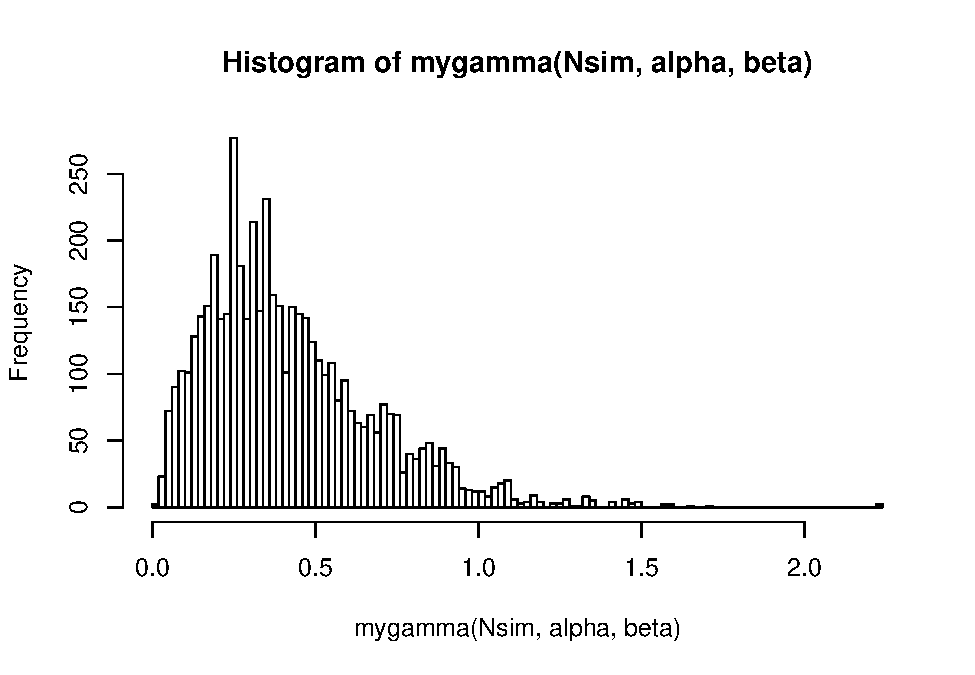
\includegraphics{bookdown-demo_files/figure-latex/unnamed-chunk-5-1.pdf}

\hypertarget{em}{%
\chapter{EM}\label{em}}

EM algorithm is an iterative method to find ML or maximum a posteriori (MAP) estimates of parameters.

Direct Ref: \url{http://www.di.fc.ul.pt/~jpn/r/EM/EM.html}

Suppose that we only observe \(X\), and do not know \(Z\). We thus need to construct the complete data of \((X, Z)\). Given \(p(Z|X,\theta)\), we can compute the likelihood of the complete dataset:

\[p(X, Z|\theta)=p(Z|X,\theta)p(X|\theta)\]
The EM algorithm:

\begin{enumerate}
\def\labelenumi{(\arabic{enumi})}
\setcounter{enumi}{-1}
\item
  We got \(X\) and \(p(Z|X,\theta)\)
\item
  Random assign a \(\theta_0\), since we do not know any of them.
\item
  E-step: \(Q_{\theta_i} = E_{Z|X,\theta_i}[log p(X,Z|\theta)]\)
\item
  M-step: compute \(\theta_{i+1} \leftarrow argmax Q_{\theta_i}\)
\item
  If \(\theta_i\) and \(\theta_{i+1}\) are not close enough, \(\theta_i \leftarrow \theta_{i+1}\). Goto step 2.
\end{enumerate}

For examples, you can refer to the following link: \url{http://www.di.fc.ul.pt/~jpn/r/EM/EM.html}

(It is em\_R.r in R\_codes folder. Personally, I can also refer to Quiz 2 in 536.)

\hypertarget{references}{%
\chapter{References}\label{references}}

\begin{enumerate}
\def\labelenumi{\arabic{enumi}.}
\tightlist
\item
  The UBC PDF about Newton
\end{enumerate}

\url{https://www.math.ubc.ca/~anstee/math104/newtonmethod.pdf}

\begin{enumerate}
\def\labelenumi{\arabic{enumi}.}
\setcounter{enumi}{1}
\tightlist
\item
  Some other pages about Newton and logistic regression
\end{enumerate}

\url{http://www.win-vector.com/blog/2011/09/the-simpler-derivation-of-logistic-regression/}

\url{https://stats.stackexchange.com/questions/344309/why-using-newtons-method-for-logistic-regression-optimization-is-called-iterati}

\url{https://tomroth.com.au/logistic/}

\url{https://www.stat.cmu.edu/~cshalizi/350/lectures/26/lecture-26.pdf}

\url{https://www.stat.cmu.edu/~cshalizi/402/lectures/14-logistic-regression/lecture-14.pdf}

\url{http://hua-zhou.github.io/teaching/biostatm280-2017spring/slides/18-newton/newton.html}

\begin{enumerate}
\def\labelenumi{\arabic{enumi}.}
\setcounter{enumi}{2}
\tightlist
\item
  MH
\end{enumerate}

\url{https://www.youtube.com/watch?v=VGRVRjr0vyw}

\hypertarget{twitter-example}{%
\chapter{Twitter Example}\label{twitter-example}}

The following is part of my course project for Stat 536. It aims to replicate part of the findings from Barbera (2015) Birds of the Same Feather Tweet Together: Bayesian Ideal Point Estimation Using Twitter Data. Political Analysis 23 (1). Note that, the following model is much simpler than that in the original paper.

\hypertarget{model}{%
\section{Model}\label{model}}

Suppose that a Twitter user is presented with a choice between following or not following another target \(j \in \{ 1, ..., m\}\). Let \(y_{j}=1\) if the user decides to follow \(j\), and \(y_{j}=0\) otherwise.

\[y_{j}=\begin{cases} 1 & Following \\ 0 & Not Following \end{cases}\]

\[p(y_{j}=1|\theta) = \frac{exp(- \theta_0|\theta_1 - x_j|^2)}{1+exp(- \theta_0|\theta_1 - x_j|^2)}\]
We additionally know the priors of \(\theta\).

\[\theta_i \sim N(0,10^2) (i = 0, 1)\]

The likelihood function is as follows.

\[L(Y|\theta)=\prod_{j=1}^{m} (\frac{exp(- \theta_0|\theta_1 - x_j|^2)}{1+exp(- \theta_0|\theta_1 - x_j|^2)})^{y_j}(1-\frac{exp(- \theta_0|\theta_1 - x_j|^2)}{1+exp(- \theta_0|\theta_1 - x_j|^2)})^{(1-y_j)}\]
Thus, the posterior is as follows.

\[L(Y|\theta) \cdot N(\theta_0|0,10) \cdot N(\theta_1|0,10)\]
\[\propto \prod_{j=1}^{m} (\frac{exp(- \theta_0|\theta_1 - x_j|^2)}{1+exp(- \theta_0|\theta_1 - x_j|^2)})^{y_j}(1-\frac{exp(- \theta_0|\theta_1 - x_j|^2)}{1+exp(- \theta_0|\theta_1 - x_j|^2)})^{(1-y_j)}\cdot exp(-\frac{1}{2}(\frac{\theta_0}{10})^2)\cdot exp(-\frac{1}{2}(\frac{\theta_1}{10})^2)\]

\begin{Shaded}
\begin{Highlighting}[]
\CommentTok{#Establish the function for logistic regression}
\NormalTok{Expit<-}\ControlFlowTok{function}\NormalTok{(x)\{}\KeywordTok{exp}\NormalTok{(x)}\OperatorTok{/}\NormalTok{(}\DecValTok{1}\OperatorTok{+}\KeywordTok{exp}\NormalTok{(x))\}}

\CommentTok{#Construct the posterior - in a log-format}
\CommentTok{#To make sure that the estimate of theta_1 is stable, }
\CommentTok{#the following code wants to make sure that theta_0 is always greater than zero.}

\NormalTok{log_post<-}\ControlFlowTok{function}\NormalTok{(Y, X, theta)}
\NormalTok{  \{}
  \ControlFlowTok{if}\NormalTok{(theta[}\DecValTok{1}\NormalTok{]}\OperatorTok{<=}\DecValTok{0}\NormalTok{)\{post=}\OperatorTok{-}\OtherTok{Inf}\NormalTok{\}}
  \ControlFlowTok{if}\NormalTok{(theta[}\DecValTok{1}\NormalTok{]}\OperatorTok{>}\DecValTok{0}\NormalTok{)\{}
\NormalTok{  prob1<-}\KeywordTok{Expit}\NormalTok{(}\OperatorTok{-}\NormalTok{theta[}\DecValTok{1}\NormalTok{]}\OperatorTok{*}\NormalTok{((theta[}\DecValTok{2}\NormalTok{]}\OperatorTok{-}\NormalTok{X)}\OperatorTok{^}\DecValTok{2}\NormalTok{))}
\NormalTok{  likelihood<-}\KeywordTok{sum}\NormalTok{(}\KeywordTok{dbinom}\NormalTok{(Y,}\DecValTok{1}\NormalTok{,prob1,}\DataTypeTok{log =} \OtherTok{TRUE}\NormalTok{))}
\NormalTok{  priors<-}\KeywordTok{sum}\NormalTok{(}\KeywordTok{dnorm}\NormalTok{(theta,}\DecValTok{0}\NormalTok{,}\DecValTok{10}\NormalTok{,}\DataTypeTok{log=}\OtherTok{TRUE}\NormalTok{))}
\NormalTok{  post=likelihood}\OperatorTok{+}\NormalTok{priors\}}
  \KeywordTok{return}\NormalTok{(post)}
\NormalTok{   \}}

\NormalTok{Bayes_logit<-}\ControlFlowTok{function}\NormalTok{ (Y,X,}\DataTypeTok{n_samples=}\DecValTok{2000}\NormalTok{)}
\NormalTok{\{}
\CommentTok{#Initial values}
\NormalTok{  theta<-}\KeywordTok{c}\NormalTok{(}\DecValTok{5}\NormalTok{,}\DecValTok{5}\NormalTok{)}
\CommentTok{#store data}
\NormalTok{  keep.theta<-}\KeywordTok{matrix}\NormalTok{(}\DecValTok{0}\NormalTok{,n_samples,}\DecValTok{2}\NormalTok{)}
\NormalTok{  keep.theta[}\DecValTok{1}\NormalTok{,]<-theta}
  
\CommentTok{#acceptance and rejection  }
\NormalTok{  acc<-att<-}\KeywordTok{rep}\NormalTok{(}\DecValTok{0}\NormalTok{,}\DecValTok{2}\NormalTok{)}
\CommentTok{#current log posterior}
\NormalTok{  current_lp<-}\KeywordTok{log_post}\NormalTok{(Y,X,theta)}

  \ControlFlowTok{for}\NormalTok{ (i }\ControlFlowTok{in} \DecValTok{2}\OperatorTok{:}\NormalTok{n_samples)  }
\NormalTok{  \{}
    
    \ControlFlowTok{for}\NormalTok{(j }\ControlFlowTok{in} \DecValTok{1}\OperatorTok{:}\DecValTok{2}\NormalTok{)}
\NormalTok{    \{}
      \CommentTok{#attempt + 1}
\NormalTok{      att[j]<-att[j]}\OperatorTok{+}\DecValTok{1}
\NormalTok{      can_theta<-theta}
\NormalTok{      can_theta[j]<-}\KeywordTok{rnorm}\NormalTok{(}\DecValTok{1}\NormalTok{,theta[j],}\FloatTok{0.5}\NormalTok{)}
      \CommentTok{#candidate of log posterior}
\NormalTok{      candidate_lp<-}\KeywordTok{log_post}\NormalTok{(Y,X,can_theta)}
\NormalTok{      Rho<-}\KeywordTok{min}\NormalTok{(}\KeywordTok{exp}\NormalTok{(candidate_lp}\OperatorTok{-}\NormalTok{current_lp),}\DecValTok{1}\NormalTok{)}
\NormalTok{      Random_probability<-}\KeywordTok{runif}\NormalTok{(}\DecValTok{1}\NormalTok{)}
      \ControlFlowTok{if}\NormalTok{ (Random_probability}\OperatorTok{<}\NormalTok{Rho)}
\NormalTok{      \{}
\NormalTok{        theta<-can_theta}
\NormalTok{        current_lp<-candidate_lp}
        \CommentTok{#acceptance + 1, as long as Random_probability<Rho}
\NormalTok{        acc[j]<-acc[j]}\OperatorTok{+}\DecValTok{1}
\NormalTok{      \}}
\NormalTok{    \}}
    \CommentTok{#save theta}
\NormalTok{    keep.theta[i,]<-theta}
\NormalTok{  \}}
\CommentTok{#Return: including theta and acceptance rate}
  \KeywordTok{list}\NormalTok{(}\DataTypeTok{theta=}\NormalTok{keep.theta,}\DataTypeTok{acceptance_rate=}\NormalTok{acc}\OperatorTok{/}\NormalTok{att)}
\NormalTok{\}}
\end{Highlighting}
\end{Shaded}

\hypertarget{simulating-data-of-senators-on-twitter}{%
\section{Simulating Data of Senators on Twitter}\label{simulating-data-of-senators-on-twitter}}

Assume that we have 100 senators, 50 Democrats and 50 Republicans, who we know their ideology. Assume that Democrats have negative ideology scores to indicate that they are more liberal, whereas Republicans have positive scores to indicate that they are more conservative. The following is data simulation for senators.

\begin{Shaded}
\begin{Highlighting}[]
\CommentTok{# Republicans are more conservative, and they have positive numbers.}
\NormalTok{Republicans<-}\KeywordTok{c}\NormalTok{()}
\NormalTok{Republicans<-}\KeywordTok{rnorm}\NormalTok{(}\DecValTok{50}\NormalTok{,}\DecValTok{1}\NormalTok{,}\FloatTok{0.5}\NormalTok{)}
\NormalTok{No_Republicans<-}\KeywordTok{rep}\NormalTok{(}\DecValTok{1}\OperatorTok{:}\DecValTok{50}\NormalTok{,}\DecValTok{1}\NormalTok{)}
\NormalTok{Part_}\DecValTok{1}\NormalTok{<-}\KeywordTok{cbind}\NormalTok{(No_Republicans,Republicans)}

\CommentTok{# Democrats are more liberal, and they have negative numbers.}
\NormalTok{Democrats<-}\KeywordTok{c}\NormalTok{()}
\NormalTok{Democrats<-}\KeywordTok{rnorm}\NormalTok{(}\DecValTok{50}\NormalTok{,}\OperatorTok{-}\DecValTok{1}\NormalTok{,}\FloatTok{0.5}\NormalTok{)}
\NormalTok{No_Democrats<-}\KeywordTok{rep}\NormalTok{(}\DecValTok{51}\OperatorTok{:}\DecValTok{100}\NormalTok{,}\DecValTok{1}\NormalTok{)}
\NormalTok{Part_}\DecValTok{2}\NormalTok{<-}\KeywordTok{cbind}\NormalTok{(No_Democrats,Democrats)}
\NormalTok{Data_Elites<-}\KeywordTok{rbind}\NormalTok{(Part_}\DecValTok{1}\NormalTok{,Part_}\DecValTok{2}\NormalTok{)}
\NormalTok{Data_Elites<-}\KeywordTok{as.data.frame}\NormalTok{(Data_Elites)}
\KeywordTok{colnames}\NormalTok{(Data_Elites) <-}\StringTok{ }\KeywordTok{c}\NormalTok{(}\StringTok{"Elite_No"}\NormalTok{,}\StringTok{"Elite_ideology"}\NormalTok{)}

\KeywordTok{head}\NormalTok{(Data_Elites)}
\end{Highlighting}
\end{Shaded}

\begin{verbatim}
##   Elite_No Elite_ideology
## 1        1      1.0541992
## 2        2      0.3805544
## 3        3      1.3568577
## 4        4      0.9922547
## 5        5      1.0089966
## 6        6      0.8878271
\end{verbatim}

\hypertarget{simulating-data-of-conservative-users-on-twitter-and-model-testing}{%
\section{Simulating Data of Conservative Users on Twitter and Model Testing}\label{simulating-data-of-conservative-users-on-twitter-and-model-testing}}

Assume that we observe one Twitter user, who is more conservative. To simulate Twitter following data for this user, I assign this user to follow more Republican senators. Thus, if the Metropolis Hastings algorithm works as intended, we would expect to see a positive estimated value for their ideology. Importantly, as we can see in the histogram below, the estimated value indeed is positive, providing preliminary evidence for the statistical model and the algorithm. In addition, for the acceptance rate, we can see that the constant has a lower number than ideology, since we only accept a constant when it is positive.

\begin{Shaded}
\begin{Highlighting}[]
\CommentTok{#This user approximately follows 45 Republican Senators and 10 Democrat Senators. }
\NormalTok{Data_user<-}\KeywordTok{as.data.frame}\NormalTok{(}\KeywordTok{matrix}\NormalTok{(}\KeywordTok{c}\NormalTok{(}\KeywordTok{ifelse}\NormalTok{(}\KeywordTok{runif}\NormalTok{(}\DecValTok{50}\NormalTok{)}\OperatorTok{<}\NormalTok{.}\DecValTok{1}\NormalTok{,}\DecValTok{0}\NormalTok{,}\DecValTok{1}\NormalTok{),}\KeywordTok{ifelse}\NormalTok{(}\KeywordTok{runif}\NormalTok{(}\DecValTok{50}\NormalTok{)}\OperatorTok{<}\NormalTok{.}\DecValTok{8}\NormalTok{,}\DecValTok{0}\NormalTok{,}\DecValTok{1}\NormalTok{))), }\DecValTok{100}\NormalTok{, }\DecValTok{1}\NormalTok{)}
\KeywordTok{colnames}\NormalTok{(Data_user)<-}\KeywordTok{c}\NormalTok{(}\StringTok{"R_User"}\NormalTok{)}
\NormalTok{Data_combined<-}\KeywordTok{cbind}\NormalTok{(Data_Elites,Data_user)}

\NormalTok{X_data<-Data_combined}\OperatorTok{$}\NormalTok{Elite_ideology}
\NormalTok{Y_data<-Data_combined}\OperatorTok{$}\NormalTok{R_User}

\NormalTok{fit_C<-}\KeywordTok{Bayes_logit}\NormalTok{(Y_data,X_data)}
\NormalTok{fit_C}\OperatorTok{$}\NormalTok{acceptance_rate}
\end{Highlighting}
\end{Shaded}

\begin{verbatim}
## [1] 0.1320660 0.5557779
\end{verbatim}

\begin{Shaded}
\begin{Highlighting}[]
\KeywordTok{plot}\NormalTok{(fit_C}\OperatorTok{$}\NormalTok{theta[,}\DecValTok{1}\NormalTok{],}\DataTypeTok{main=}\StringTok{"Constant (Conservative Users)"}\NormalTok{,}
     \DataTypeTok{xlab=}\StringTok{"Iteration Process"}\NormalTok{,}\DataTypeTok{ylab=}\StringTok{"Estimated Scores"}\NormalTok{,}\DataTypeTok{type=}\StringTok{"l"}\NormalTok{)}
\end{Highlighting}
\end{Shaded}

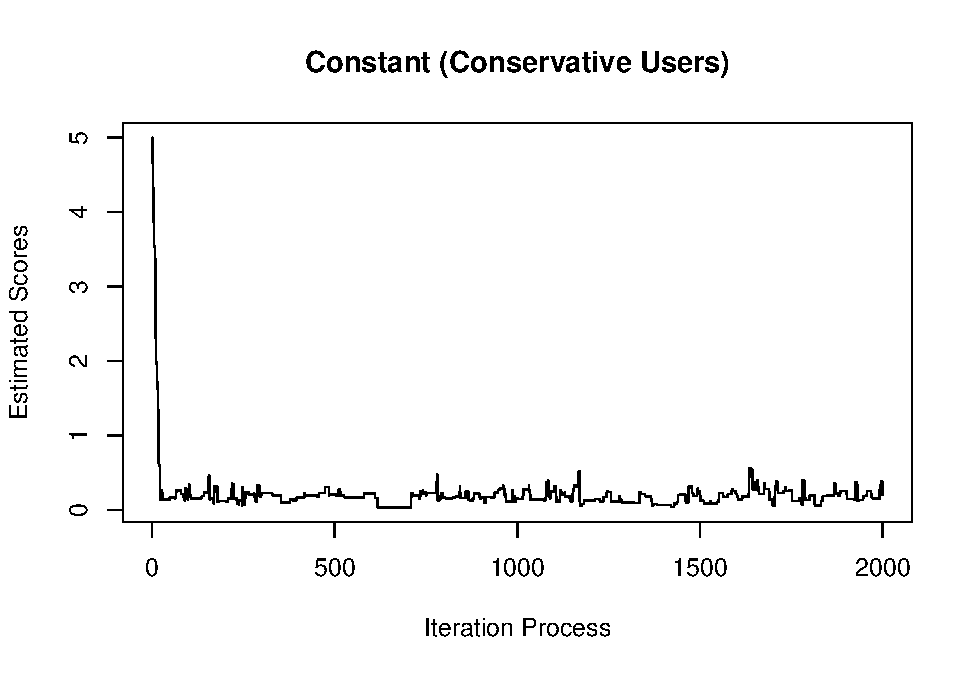
\includegraphics{bookdown-demo_files/figure-latex/unnamed-chunk-8-1.pdf}

\begin{Shaded}
\begin{Highlighting}[]
\KeywordTok{plot}\NormalTok{(fit_C}\OperatorTok{$}\NormalTok{theta[,}\DecValTok{2}\NormalTok{],}\DataTypeTok{main=}\StringTok{"Estimated Ideology Scores (Conservative Users)"}\NormalTok{,}
     \DataTypeTok{xlab=}\StringTok{"Iteration Process"}\NormalTok{,}\DataTypeTok{ylab=}\StringTok{"Ideology Scores"}\NormalTok{,}\DataTypeTok{type=}\StringTok{"l"}\NormalTok{)}
\end{Highlighting}
\end{Shaded}

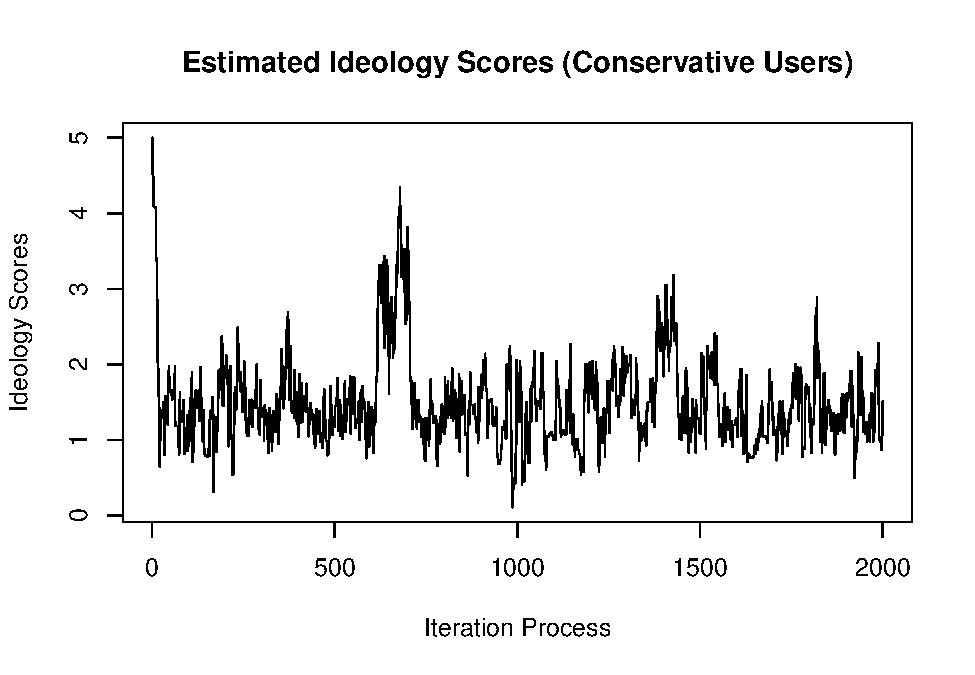
\includegraphics{bookdown-demo_files/figure-latex/unnamed-chunk-8-2.pdf}

\begin{Shaded}
\begin{Highlighting}[]
\KeywordTok{hist}\NormalTok{(fit_C}\OperatorTok{$}\NormalTok{theta[,}\DecValTok{2}\NormalTok{],}\DataTypeTok{main=}\StringTok{"Estimated Ideology Scores (Conservative Users)"}\NormalTok{,}
     \DataTypeTok{xlab=}\StringTok{"Ideology Scores"}\NormalTok{,}\DataTypeTok{breaks =} \DecValTok{100}\NormalTok{)}
\end{Highlighting}
\end{Shaded}

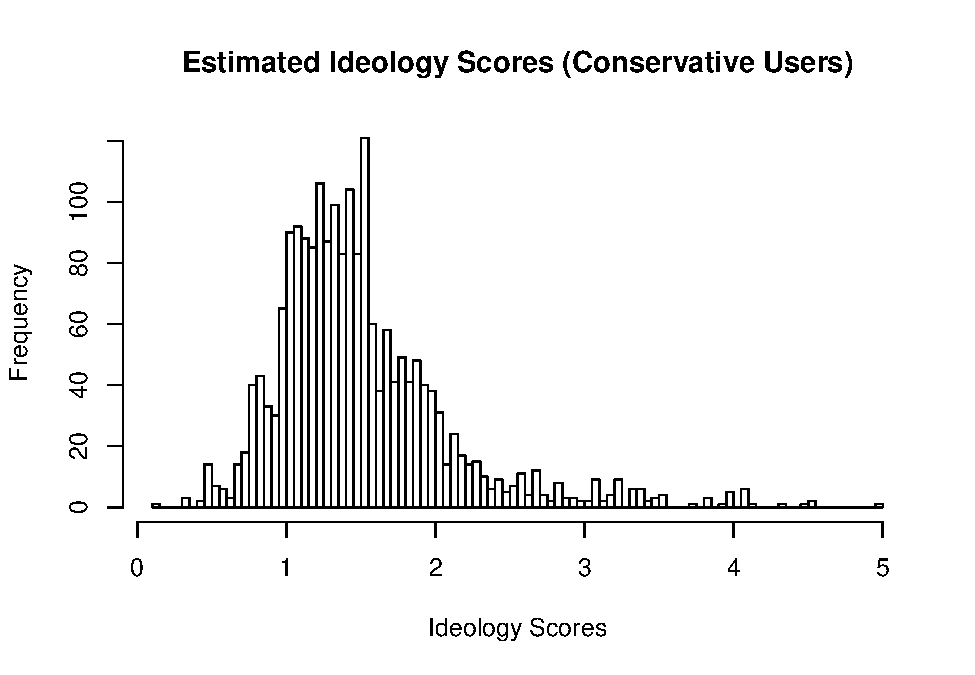
\includegraphics{bookdown-demo_files/figure-latex/unnamed-chunk-8-3.pdf}

\hypertarget{simulating-data-of-liberal-users-on-twitter-and-model-testing}{%
\section{Simulating Data of Liberal Users on Twitter and Model Testing}\label{simulating-data-of-liberal-users-on-twitter-and-model-testing}}

To further verify the Metropolis Hastings algorithm, I plan to test the opposite estimate. Specifically, assume that we observe another user, who is more liberal. To simulate Twitter following data for this user, I assign this user to follow more Democrat senators. In this case, we would expect to see a negative value for their estimated ideology. As we can see in the histogram shown below, as expected, the estimated value is negative, providing convergent evidence for the model and the algorithm.

\begin{Shaded}
\begin{Highlighting}[]
\CommentTok{#This user approximately follows 10 Republican Senators and 45 Democrat Senators. }
\NormalTok{Data_user<-}\KeywordTok{as.data.frame}\NormalTok{(}\KeywordTok{matrix}\NormalTok{(}\KeywordTok{c}\NormalTok{(}\KeywordTok{ifelse}\NormalTok{(}\KeywordTok{runif}\NormalTok{(}\DecValTok{50}\NormalTok{)}\OperatorTok{<}\NormalTok{.}\DecValTok{8}\NormalTok{,}\DecValTok{0}\NormalTok{,}\DecValTok{1}\NormalTok{),}\KeywordTok{ifelse}\NormalTok{(}\KeywordTok{runif}\NormalTok{(}\DecValTok{50}\NormalTok{)}\OperatorTok{<}\NormalTok{.}\DecValTok{1}\NormalTok{,}\DecValTok{0}\NormalTok{,}\DecValTok{1}\NormalTok{))), }\DecValTok{100}\NormalTok{, }\DecValTok{1}\NormalTok{)}
\KeywordTok{colnames}\NormalTok{(Data_user)<-}\KeywordTok{c}\NormalTok{(}\StringTok{"L_User"}\NormalTok{)}
\NormalTok{Data_combined<-}\KeywordTok{cbind}\NormalTok{(Data_Elites,Data_user)}

\NormalTok{X_data<-Data_combined}\OperatorTok{$}\NormalTok{Elite_ideology}
\NormalTok{Y_data<-Data_combined}\OperatorTok{$}\NormalTok{L_User}


\NormalTok{fit_L<-}\KeywordTok{Bayes_logit}\NormalTok{(Y_data,X_data)}
\NormalTok{fit_L}\OperatorTok{$}\NormalTok{acceptance_rate}
\end{Highlighting}
\end{Shaded}

\begin{verbatim}
## [1] 0.1585793 0.5092546
\end{verbatim}

\begin{Shaded}
\begin{Highlighting}[]
\KeywordTok{plot}\NormalTok{(fit_L}\OperatorTok{$}\NormalTok{theta[,}\DecValTok{1}\NormalTok{],}\DataTypeTok{main=}\StringTok{"Constant (Liberal Users)"}\NormalTok{,}
     \DataTypeTok{xlab=}\StringTok{"Iteration Process"}\NormalTok{,}\DataTypeTok{ylab=}\StringTok{"Estimated Scores"}\NormalTok{,}\DataTypeTok{type=}\StringTok{"l"}\NormalTok{)}
\end{Highlighting}
\end{Shaded}

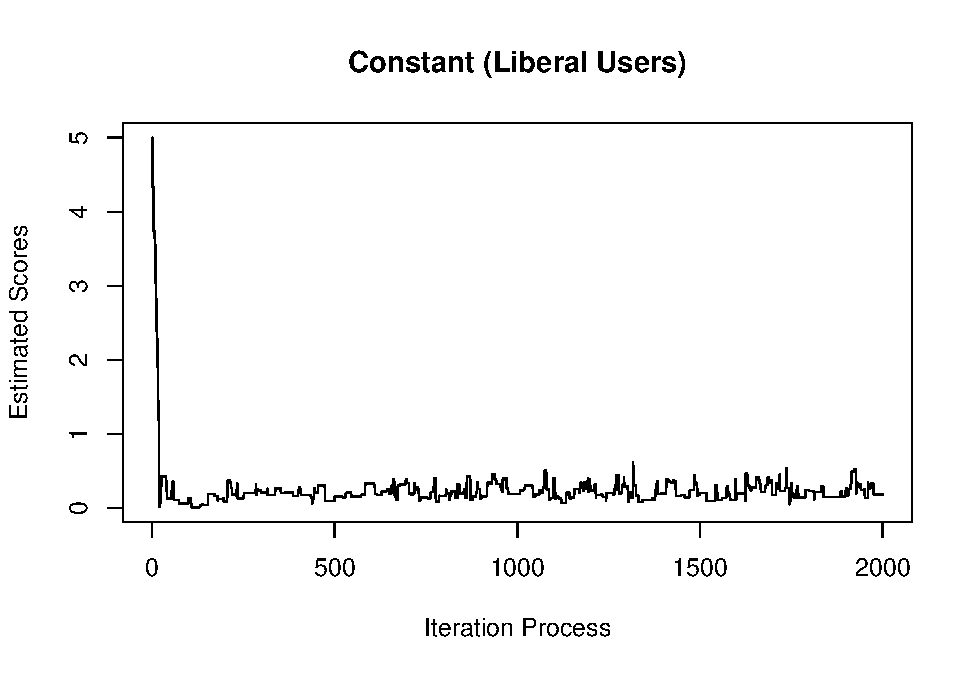
\includegraphics{bookdown-demo_files/figure-latex/unnamed-chunk-9-1.pdf}

\begin{Shaded}
\begin{Highlighting}[]
\KeywordTok{plot}\NormalTok{(fit_L}\OperatorTok{$}\NormalTok{theta[,}\DecValTok{2}\NormalTok{],}\DataTypeTok{main=}\StringTok{"Estimated Ideology Scores (Liberal Users)"}\NormalTok{,}
     \DataTypeTok{xlab=}\StringTok{"Iteration Process"}\NormalTok{,}\DataTypeTok{ylab=}\StringTok{"Ideology Scores"}\NormalTok{,}\DataTypeTok{type=}\StringTok{"l"}\NormalTok{)}
\end{Highlighting}
\end{Shaded}

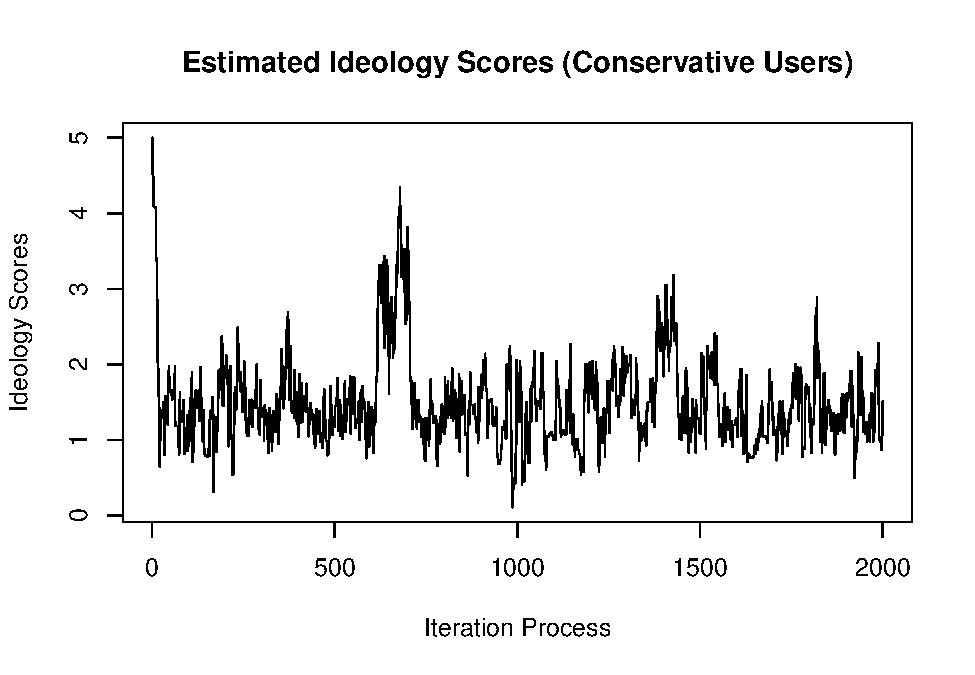
\includegraphics{bookdown-demo_files/figure-latex/unnamed-chunk-9-2.pdf}

\begin{Shaded}
\begin{Highlighting}[]
\KeywordTok{hist}\NormalTok{(fit_L}\OperatorTok{$}\NormalTok{theta[,}\DecValTok{2}\NormalTok{],}\DataTypeTok{main=}\StringTok{"Estimated Ideology Scores (Liberal Users)"}\NormalTok{,}
     \DataTypeTok{xlab=}\StringTok{"Ideology Scores"}\NormalTok{,}\DataTypeTok{breaks =} \DecValTok{100}\NormalTok{)}
\end{Highlighting}
\end{Shaded}

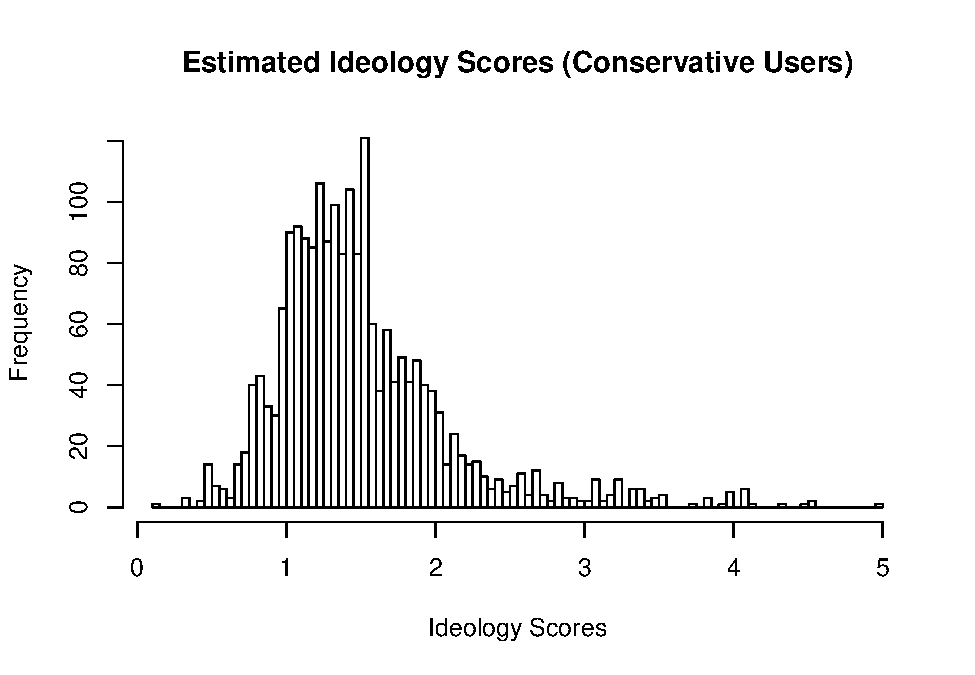
\includegraphics{bookdown-demo_files/figure-latex/unnamed-chunk-9-3.pdf}

\backmatter
  \bibliography{book.bib,packages.bib}

\end{document}
